
\usetikzlibrary{calc}
\usetikzlibrary{chains, decorations.pathreplacing, positioning}

\definecolor{decoration}{RGB}{0, 122, 195} %CTU blue
\definecolor{heading}{RGB}{0, 122, 195}
\definecolor{headbackgroundgray}{RGB}{199, 219, 241} %light blue
\definecolor{backgroundgray}{RGB}{199, 219, 241} %CTU light blue
\definecolor{headgray}{rgb}{0.50,0.50,0.51}
\definecolor{enumgray}{RGB}{0, 122, 195} %CTU blue

\begin{figure}[h]
  \caption{The edge index layout in two-dimensional grid}
  \label{fig:memory-1-D}

  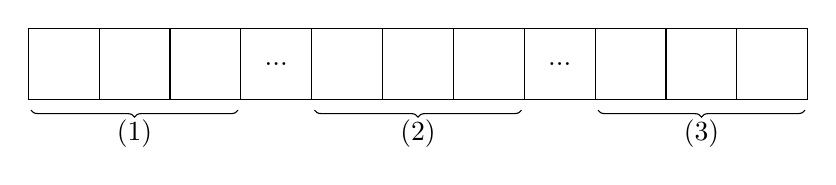
\begin{tikzpicture}[scale=0.9]
    \draw (0,0) grid (11,1);

    \draw [decorate, decoration = {brace, mirror, raise = 4pt}] (0.04, 0,0) -- (2.96, 0) node[pos=0.5,below=4pt,black] {(1)};
    \draw [decorate, decoration = {brace, mirror, raise = 4pt}] (4.04, 0,0) -- (6.96, 0) node[pos=0.5,below=4pt,black] {(2)};
    \draw [decorate, decoration = {brace, mirror, raise = 4pt}] (8.04, 0,0) -- (10.96, 0) node[pos=0.5,below=4pt,black] {(3)};

    \node[label] at (3.5,0.5) {...};
    \node[label] at (7.5,0.5) {...};
  \end{tikzpicture}
\end{figure}